\documentclass[
	a4paper,
	oneside,
	BCOR = 10mm,
	DIV = 12,
	12pt,
	headings = normal,
]{scrartcl}

%%% Length calculations
\usepackage{calc}
%%%

%%% Support for color
\usepackage{xcolor}
\definecolor{lightblue}{HTML}{03A9F4}
\definecolor{red}{HTML}{F44336}
%%%

%%% Including graphics
\usepackage{graphicx}
%%%

%%% Font selection
\usepackage{fontspec}

\setromanfont{STIX Two Text}[
	SmallCapsFeatures = {LetterSpace = 8},
]

\setsansfont{IBM Plex Sans}[
	Scale = MatchUppercase,
]

\setmonofont{IBM Plex Mono}[
	Scale = MatchUppercase,
]
%%%

%%% Math typesetting
\usepackage{amsmath}

\usepackage{unicode-math}
\setmathfont{STIX Two Math}

\usepackage{IEEEtrantools}
%%%

%%% List settings
\usepackage{enumitem}
\setlist[enumerate]{
	label*      = {\arabic*.},
	left        = \parindent,
	topsep      = 0\baselineskip,
	parsep      = 0\baselineskip,
	noitemsep, % override itemsep
}
% List settings for levels 2–4
\setlist[enumerate, 2, 3, 4]{
	label*      = {\arabic*.},
	left        = 0em,
	topsep      = 0\baselineskip,
	parsep      = 0\baselineskip,
	noitemsep, % override itemsep
}

\setlist[itemize]{
	label*      = {—},
	left        = \parindent,
	topsep      = 0\baselineskip,
	parsep      = 0\baselineskip,
	itemsep     = 1\baselineskip,
	noitemsep, % override itemsep
}

\setlist[description]{
	font        = {\rmfamily\upshape\bfseries},
	topsep      = 1\baselineskip,
	parsep      = 0\baselineskip,
	itemsep     = 0\baselineskip,
}

%%%

%%% Structural elements typesetting
\setkomafont{pagenumber}{\rmfamily\upshape}
\setkomafont{disposition}{\rmfamily\bfseries}

% Sectioning
\RedeclareSectionCommand[
	beforeskip = -1\baselineskip,
	afterskip  = 1\baselineskip,
	font       = {\normalsize\bfseries\scshape},
]{section}

\RedeclareSectionCommand[
	beforeskip = -1\baselineskip,
	afterskip  = 1\baselineskip,
	font       = {\normalsize\bfseries\itshape},
]{subsection}

\RedeclareSectionCommand[
	beforeskip = -1\baselineskip,
	afterskip  = 1\baselineskip,
	font       = {\normalsize\bfseries},
]{subsubsection}

\RedeclareSectionCommand[
	beforeskip = -1\baselineskip,
	afterskip  = -0.5em,
	font       = {\normalsize\mdseries\scshape\addfontfeatures{Letters = {UppercaseSmallCaps}}},
]{paragraph}
%%%

%%% Typographic enhancements
\usepackage{microtype}
%%%

%%% Language-specific settings
\usepackage{polyglossia}
\setmainlanguage{ukrainian}
\setotherlanguages{english}
%%%

%%% Captions
\usepackage{caption}
\usepackage{subcaption}

%\DeclareCaptionLabelFormat{closing}{#2)}
%\captionsetup[subtable]{labelformat = closing}

%\captionsetup[subfigure]{labelformat = closing}

\captionsetup[table]{
	aboveskip = 0\baselineskip,
	belowskip = 0\baselineskip,
}

\captionsetup[figure]{
	aboveskip = 1\baselineskip,
	belowskip = 0\baselineskip,
}

\captionsetup[subfigure]{
	labelformat = simple,
	labelformat = brace,
}
%%%

%%% Hyphenated ragged typesetting
\usepackage{ragged2e}
%%%

%%% Table typesetting
\usepackage{booktabs}
\usepackage{longtable}

\usepackage{multirow}

\usepackage{array}
\newcolumntype{v}[1]{>{\RaggedRight\arraybackslash\hspace{0pt}}p{#1}}
\newcolumntype{b}[1]{>{\Centering\arraybackslash\hspace{0pt}}p{#1}}
\newcolumntype{n}[1]{>{\RaggedLeft\arraybackslash\hspace{0pt}}p{#1}}
%%%

%%% Drawing
\usepackage{tikz}
\usepackage{tikzscale}
\usetikzlibrary{positioning}
\usetikzlibrary{arrows.meta} % Stealth arrow tips
%%%

%%% SI units typesetting
\usepackage{siunitx}
\sisetup{
	output-decimal-marker = {,},
	exponent-product      = {\cdot},
	inter-unit-product    = \ensuremath{{} \cdot {}},
	per-mode              = symbol,
}
%%%

% Code Highlighting
\usepackage{minted}
\setmintedinline{
	style = bw,
	breaklines,
}

\newminted[bashterm]{bash}{%
	autogobble,%
	style=bw,%
}

\newminted[codegeneric]{text}{%
	autogobble,%
	style=bw,%
	breaklines,%
	fontsize=\small,%
}

\newmintinline{bash}{%
}

\newmintinline[minttext]{text}{%
	breaklines,%
}

\newmintinline[acad]{text}{%
	breaklines,%
}

%%% Framing code listings
\usepackage{tcolorbox}
\tcbuselibrary{breakable}
\tcbuselibrary{minted}
\tcbuselibrary{skins}

% Text file listing
\newtcblisting[
	auto counter,
	list inside,
	number within = section,
]{listingplaintext}[3][]{%
	minted language = text,
	minted style    = bw,
	minted options  = {
		autogobble,
		linenos,
		tabsize = 4,
		breaklines,
		breakanywhere,
		fontsize = \footnotesize,
	},
	empty,
	sharp corners,
	coltitle = black,
	borderline horizontal = {1pt}{0pt}{black},
	titlerule = {0.5pt},
	titlerule style = {
		black,
	},
	toptitle = 0.3em,
	bottomtitle = 0.3em,
	before skip      = \intextsep,
	after  skip      = \intextsep,
	title            = {Лістинг \thetcbcounter: #2},
	list entry       = {\protect\numberline{\thetcbcounter}#2},
	left = 0em,
	right = 0em,
	%
	listing only,
	breakable,
	%
	label = {#3},%
}

\newtcblisting[
	use counter from = listingplaintext,
	list inside,
	number within = section,
]{listingpython}[3][]{%
	minted language = python,
	minted style    = bw,
	minted options  = {
		autogobble,
		linenos,
		tabsize = 4,
		breaklines,
		breakanywhere,
		fontsize = \footnotesize,
	},
	empty,
	sharp corners,
	coltitle = black,
	borderline horizontal = {1pt}{0pt}{black},
	titlerule = {0.5pt},
	titlerule style = {
		black,
	},
	toptitle = 0.3em,
	bottomtitle = 0.3em,
	before skip      = \intextsep,
	after  skip      = \intextsep,
	title            = {Лістинг \thetcbcounter: #2},
	list entry       = {\protect\numberline{\thetcbcounter}#2},
	left = 0em,
	right = 0em,
	%
	listing only,
	breakable,
	%
	label = {#3},
	%
	#1%
}

\newtcbinputlisting[
	use counter from = listingplaintext,
	list inside,
	number within = section
]{\inputpython}[4][]{%
	minted language = python,
	minted style    = bw,
	minted options  = {
		autogobble,
		linenos,
		tabsize = 4,
		breaklines,
		breakanywhere,
		fontsize = \footnotesize,
	},
	empty,
	sharp corners,
	coltitle = black,
	borderline horizontal = {1pt}{0pt}{black},
	titlerule = {0.5pt},
	titlerule style = {
		black,
	},
	toptitle = 0.3em,
	bottomtitle = 0.3em,
	before skip      = \intextsep,
	after  skip      = \intextsep,
	title            = {Лістинг \thetcbcounter: #3},
	list entry       = {\protect\numberline{\thetcbcounter}#3},
	left = 0em,
	right = 0em,
	%
	listing file={#2},
	listing only,
	breakable,
	%
	label = {#4}
}

% Linux command-line listing
\newtcblisting{linuxterm}%
{%
	% Syntax highlighing options
	listing only,%
	minted language = bash,%
	minted options={%
		autogobble,%
		linenos%
	},%
	% Presentation options
	empty,%
	%% Margins
	sharp corners,%
	toptitle = 0.0em,%
	bottomtitle = 0.0em,%
	left = 0em,%
	right = 0em,%
	before skip = \intextsep,%
	after skip = \intextsep,%
}

\newtcblisting{linuxtermout}%
{%
	% Syntax highlighing options
	listing only,%
	minted language = text,%
	minted options={%
		autogobble,%
		linenos%
	},%
	% Presentation options
	empty,%
	%% Margins
	sharp corners,%
	toptitle = 0.0em,%
	bottomtitle = 0.0em,%
	left = 0em,%
	right = 0em,%
	before skip = \intextsep,%
	after skip = \intextsep,%
}

% Dockerfile listings
\newtcblisting[
	use counter from = listingplaintext,
	list inside,
	number within = section,
]{listingdocker}[3][]{%
	minted language = dockerfile,
	minted style    = bw,
	minted options  = {
		autogobble,%
		linenos,
		tabsize = 4,
		breaklines,
		breakanywhere,
		fontsize = \footnotesize,
	},
	empty,
	sharp corners,
	coltitle = black,
	borderline horizontal = {1pt}{0pt}{black},
	titlerule = {0.5pt},
	titlerule style = {
		black,
	},
	toptitle = 0.3em,
	bottomtitle = 0.3em,
	before skip      = \intextsep,
	after  skip      = \intextsep,
	title            = {Лістинг \thetcbcounter: #2},
	list entry       = {\protect\numberline{\thetcbcounter}#2},
	left = 0em,
	right = 0em,
	%
	listing only,
	breakable,
	%
	label = {#3},%
}

% Docker Compose listings
\newtcblisting[
	use counter from = listingplaintext,
	list inside,
	number within = section,
]{listingdockercompose}[3][]{%
	minted language = yaml,
	minted style    = bw,
	minted options  = {
		autogobble,%
		linenos,
		tabsize = 4,
		breaklines,
		breakanywhere,
		fontsize = \footnotesize,
	},
	empty,
	sharp corners,
	coltitle = black,
	borderline horizontal = {1pt}{0pt}{black},
	titlerule = {0.5pt},
	titlerule style = {
		black,
	},
	toptitle = 0.3em,
	bottomtitle = 0.3em,
	before skip      = \intextsep,
	after  skip      = \intextsep,
	title            = {Лістинг \thetcbcounter: #2},
	list entry       = {\protect\numberline{\thetcbcounter}#2},
	left = 0em,
	right = 0em,
	%
	listing only,
	breakable,
	%
	label = {#3},%
}


% Customize minted line numbers
\renewcommand{\theFancyVerbLine}{\ttfamily\scriptsize\arabic{FancyVerbLine}}

%%%

%%% Typeset menus and keys
\usepackage{menukeys}[
	os=win,
]
%%%

%%% Including full PDF documents
\usepackage{pdfpages}
%%%

%%% Links and hyperreferences
\usepackage{hyperref}
\hypersetup{
	bookmarksnumbered = true,
	colorlinks      = false,
	linkbordercolor = red,
	urlbordercolor  = lightblue,
	pdfborderstyle  = {/S/U/W 1.5},
}
%%%

%%% Length adjustment

% Set baselineskip, default is 14.5 pt
\linespread{1.068966} % ~15.5 pt
\setlength{\emergencystretch}{1em}
\setlength{\parindent}{1.5em}
\newlength{\gridunitwidth}
\setlength{\gridunitwidth}{\textwidth / 12}
%%%

%%% Custom commands
\newcommand{\allcaps}[1]{%
	{%
		\addfontfeatures{%
			Letters = UppercaseSmallCaps,
			LetterSpace = 8,%
		}%
		#1%
	}%
}
\newcommand{\filename}[1]{\texttt{#1}}
\newcommand{\progname}[1]{\texttt{#1}}
\newcommand{\commandname}[1]{\texttt{#1}}
\newcommand{\modulename}[1]{\texttt{#1}}
\newcommand{\transeng}[1]{{англ.}~\textit{\textenglish{#1}}}
%%%

%%% Custom math commands
\newcommand{\longvar}[1]{\mathit{#1}}
%%%

\begin{document}

\begin{titlepage}
		\begin{center}
			Міністерство освіти і~науки України\\
			Національний авіаційний університет\\
			Факультет кібербезпеки, комп'ютерної та програмної інженерії\\
			Кафедра комп'ютеризованих систем управління

			\vspace{\fill}
				Лабораторна робота №~1.3\\
				з~дисципліни «Технології проектування комп'ютерних систем»\\
				на~тему «Тривимірні побудови»\\
				Варіант №~8

			\vspace{\fill}

			\begin{flushright}
				Виконав:\\
				студент \allcaps{ФККПІ}\\
				групи \allcaps{СП}-425\\
				Клокун В.\,Д.\\
				Перевірила:\\
				Голего Н.\,М.
			\end{flushright}

			Київ 2019
		\end{center}
	\end{titlepage}

	\section{Мета роботи}
		Оволодіти технологіями відображення графічних об'єктів у тривимірному вигляді.

	\section{Хід~роботи}
		\subsection{Побудова вихідного зображення сітки}
			Створюємо клітинку сітки. Для цього виконуємо таку команду:
			\begin{codegeneric}
					Command: rectangle
					Specify first corner point or [Chamfer/Elevation/Fillet/Thickness/Width]: 0,0
					Specify other corner point or [Area/Dimensions/Rotation]: 10,10
			\end{codegeneric}
			Після виконання команди побудували необхідну клітинку~(рис.~\ref{subfig:01-grid-cell}). Далі будуємо сітку з клітинок розміром~$12 \times 12$. Для цього виділяємо створену клітинку, викликаємо команду~\acad{array} і задаємо бажані налаштування~(рис.~\ref{subfig:01-grid-cell-array}). Натискаємо кнопку «ОК» і отримуємо сітку~(рис.~\ref{subfig:01-grid}).

			\begin{figure}[!htbp]
				\begin{subfigure}[b]{4 \gridunitwidth - (2em / 3)}
					% \centering
					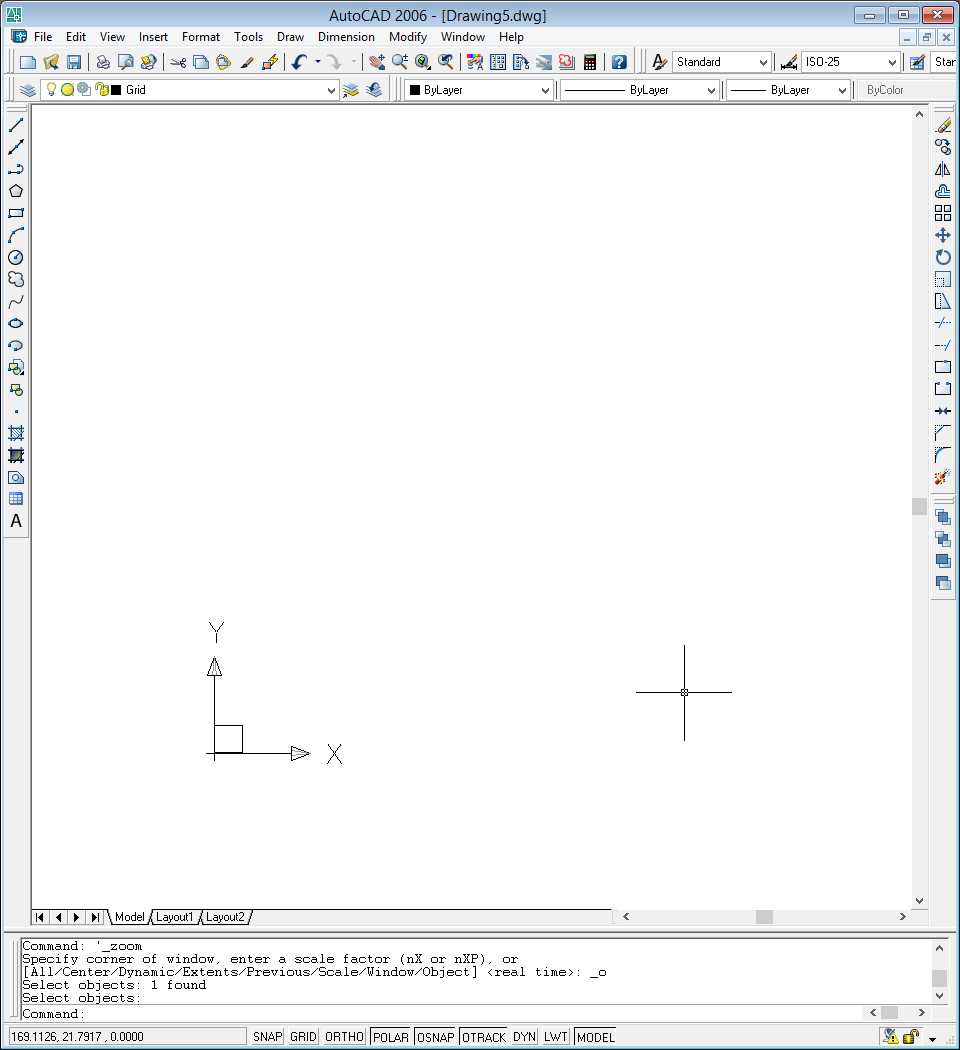
\includegraphics[width = \columnwidth]{./assets/p01.png}
					\caption{}
					\label{subfig:01-grid-cell}
				\end{subfigure}%
				\hspace{1em}%
				\begin{subfigure}[b]{4 \gridunitwidth - (2em / 3)}
					\centering
					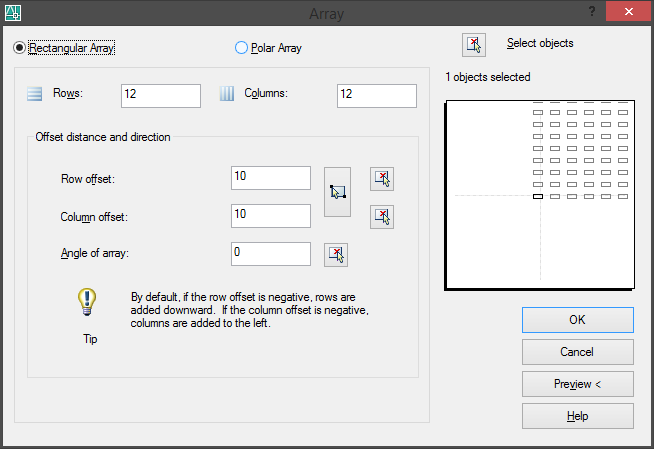
\includegraphics[width = \columnwidth]{./assets/p02.png}
					\caption{}
					\label{subfig:01-grid-cell-array}
				\end{subfigure}%
				\hspace{1em}%
				\begin{subfigure}[b]{4 \gridunitwidth - (2em / 3)}
					\centering
					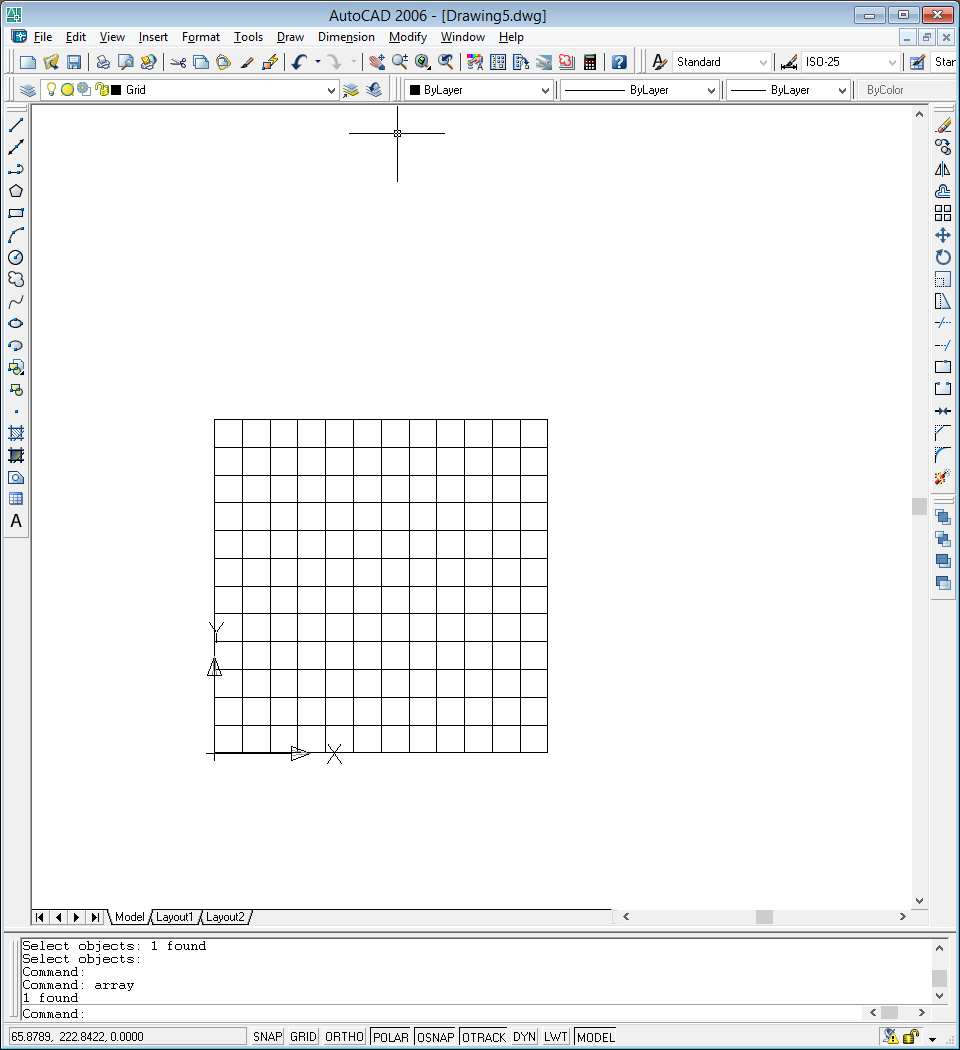
\includegraphics[width = \columnwidth]{./assets/p03.png}
					\caption{}
					\label{subfig:01-grid}
				\end{subfigure}
				\caption{Побудова сітки}
				\label{fig:01-grid-construction}
			\end{figure}

			Отже, в результаті виконання вправи ми побудували вихідне зображення сітки за допомогою команд~\acad{rectangle} і \acad{array}.

		\subsection{Побудова вихідного зображення фігур}
			Необхідно побудувати вихідні зобреження многокутника, кола і трикутника. Щоб побудувати многокутник, викликаємо команду~\acad{pline} і вказуємо точки, в яких знаходяться його кути~(рис.~\ref{subfig:02-figures-polygon}). Щоб побудувати коло, викликаємо команду~\acad{circle}, вказуємо центр кола, а потім радіус~(рис.~\ref{subfig:02-figures-circle}). Щоб побудувати трикутник, викликаємо команду~\acad{pline} і вказуємо три точки, які визначають бажаний трикутник~(рис.~\ref{subfig:02-figures-triangle}).

			\begin{figure}[!htbp]
				\begin{subfigure}[b]{6 \gridunitwidth - (1em / 2)}
					% \centering
					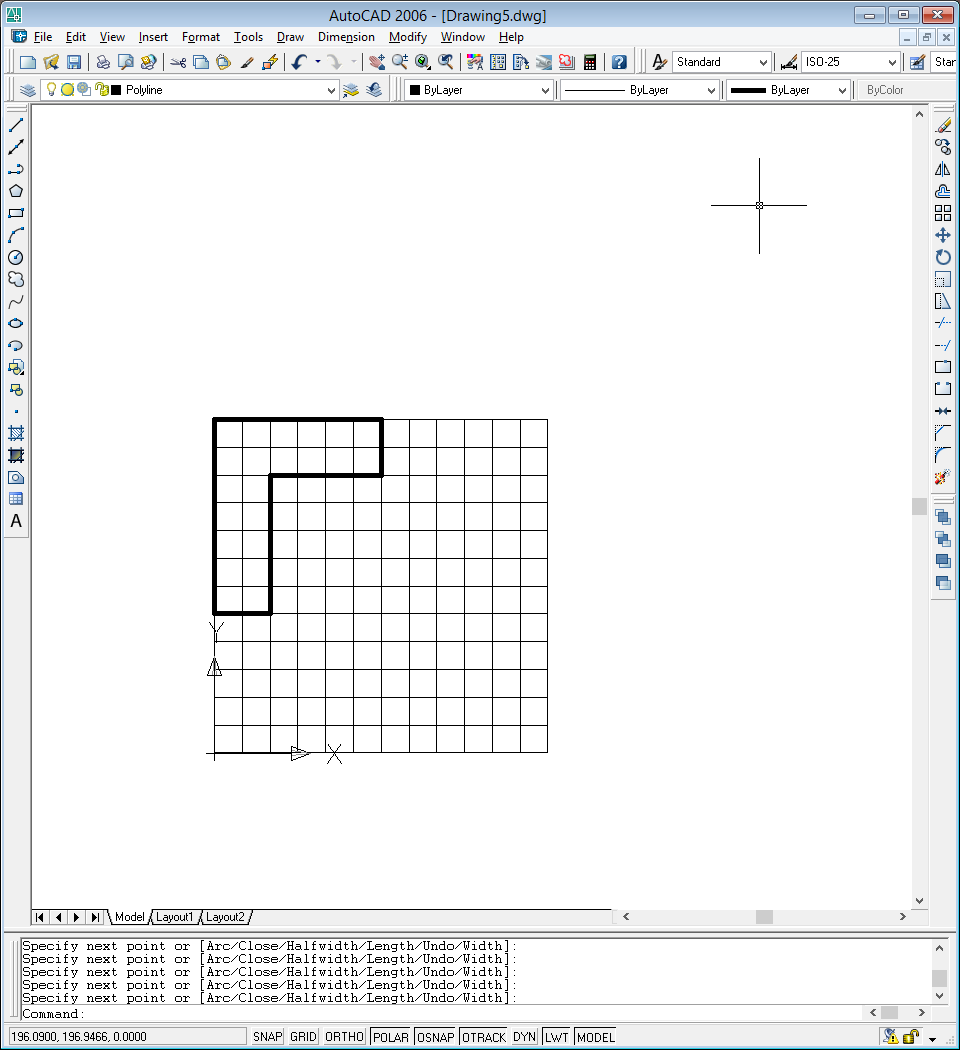
\includegraphics[width = \columnwidth]{./assets/p04.png}
					\caption{}
					\label{subfig:02-figures-polygon}
				\end{subfigure}%
				\hspace{1em}%
				\begin{subfigure}[b]{6 \gridunitwidth - (1em / 2)}
					\centering
					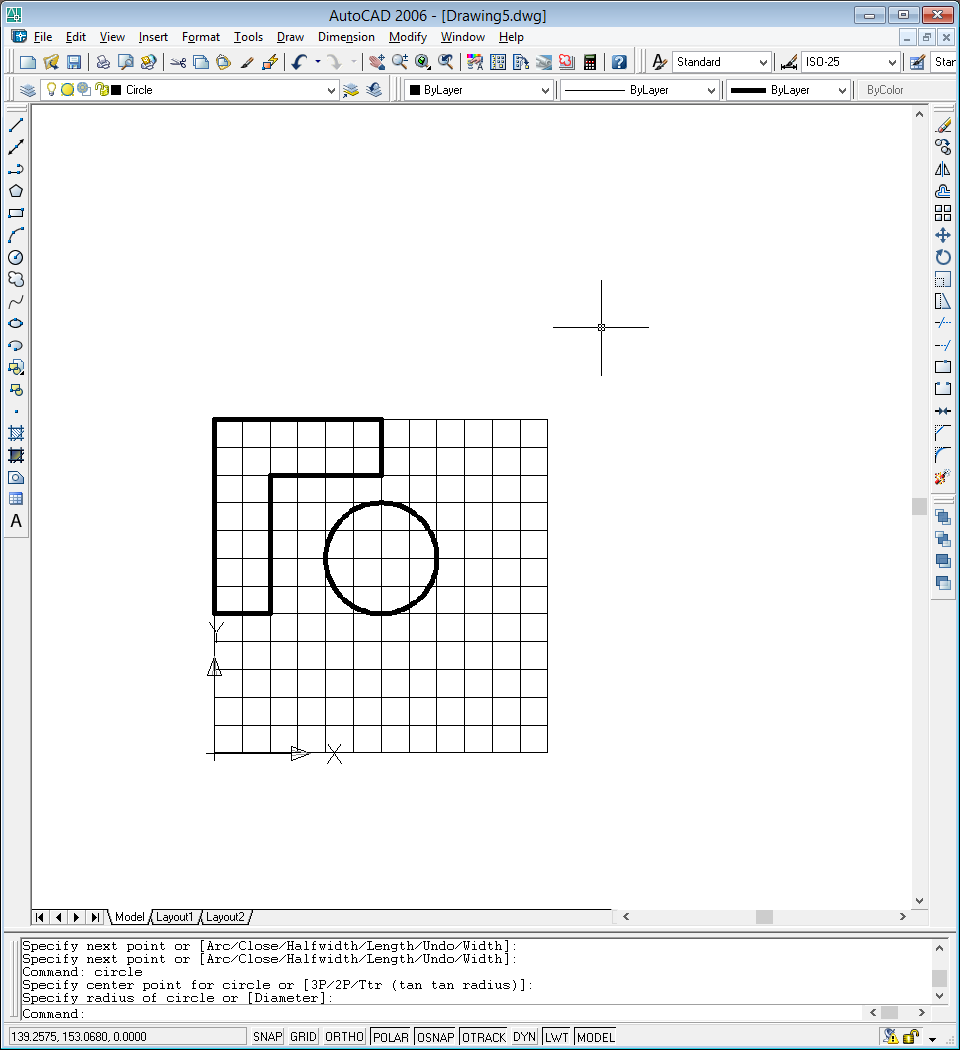
\includegraphics[width = \columnwidth]{./assets/p05.png}
					\caption{}
					\label{subfig:02-figures-circle}
				\end{subfigure}%
				\hspace{1em}%
				\begin{subfigure}[b]{6 \gridunitwidth - (1em / 2)}
					\centering
					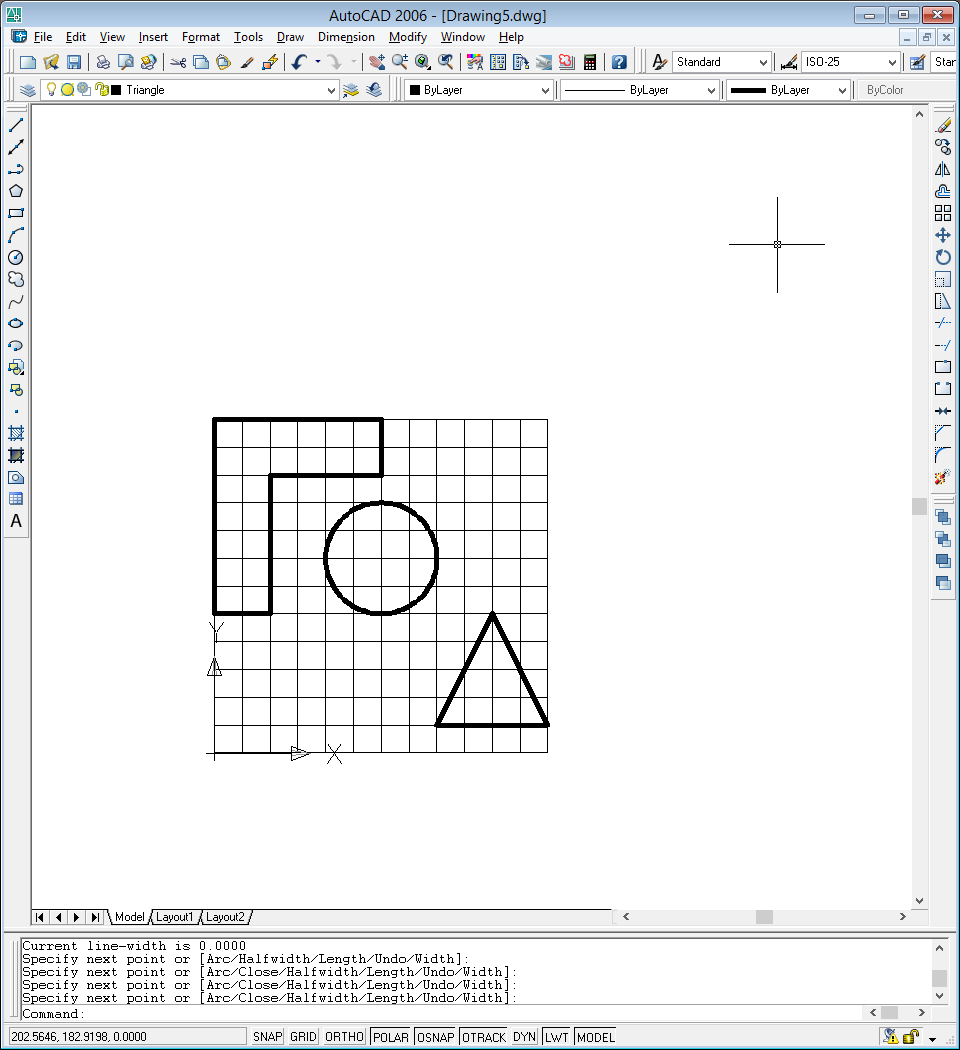
\includegraphics[width = \columnwidth]{./assets/p06.png}
					\caption{}
					\label{subfig:02-figures-triangle}
				\end{subfigure}
				\caption{Побудова вихідних зображень фігур}
				\label{fig:02-figures}
			\end{figure}

			Отже, в результаті виконання вправи ми побудували вихідні зображення багатокутника, кола і трикутника за допомогою команд~\acad{pline} і \acad{circle}.

		\subsection{Установка режиму тривимірних фігур}
			Щоб установити режим тривимірних фігур, використаємо ізометричне представлення. Для цього вибираємо пункт меню~\menu{\textenglish{3D Views} > \textenglish{SE Isometric}}. В результаті отримаємо ізометричне представлення побудованих плоских фігур~(рис.~\ref{subfig:03-figures-3d-iso-se}). Далі надаємо фігурам об'єму, для цього обираємо бажану фігуру, відкриваємо вікно~\textenglish{«Properties»} і встановлюємо ненульове значення параметру~\textenglish{Thickness}~(рис.~\ref{subfig:03-figures-3d-tall-polygon}). Повторюємо процес для всіх побудованих фігур~(рис.~\ref{subfig:03-figures-3d-tall-all}). Потім сховаємо фігури залежно від кута огляду~(рис.~\ref{subfig:03-figures-3d-hidden}). Для цього вибираємо пункт меню~\menu{\textenglish{View} > \textenglish{Hide}}.

			\begin{figure}[!htbp]
				\begin{subfigure}[b]{4 \gridunitwidth}
					% \centering
					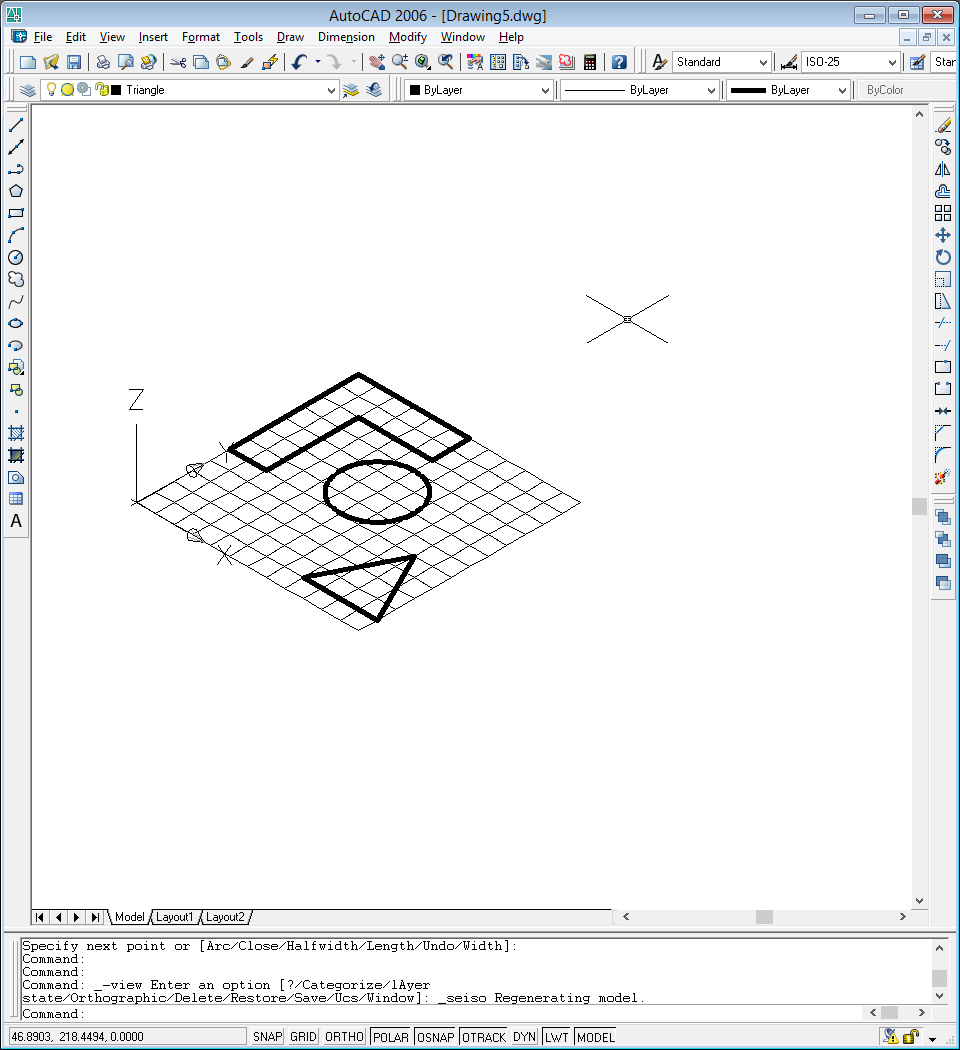
\includegraphics[width = \columnwidth]{./assets/p07.png}
					\caption{}
					\label{subfig:03-figures-3d-iso-se}
				\end{subfigure}%
				\hspace{2 \gridunitwidth}%
				\begin{subfigure}[b]{4 \gridunitwidth}
					\centering
					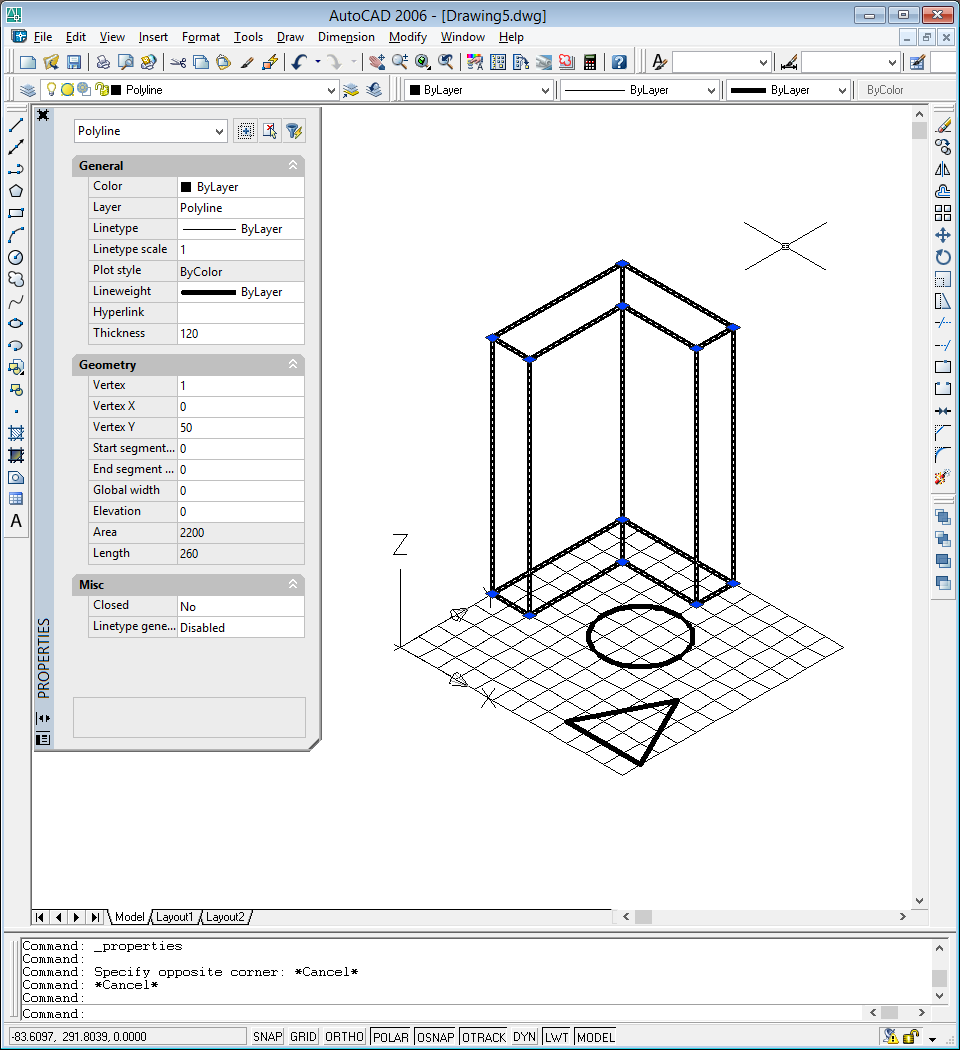
\includegraphics[width = \columnwidth]{./assets/p08.png}
					\caption{}
					\label{subfig:03-figures-3d-tall-polygon}
				\end{subfigure}
				\begin{subfigure}[b]{4 \gridunitwidth}
					\centering
					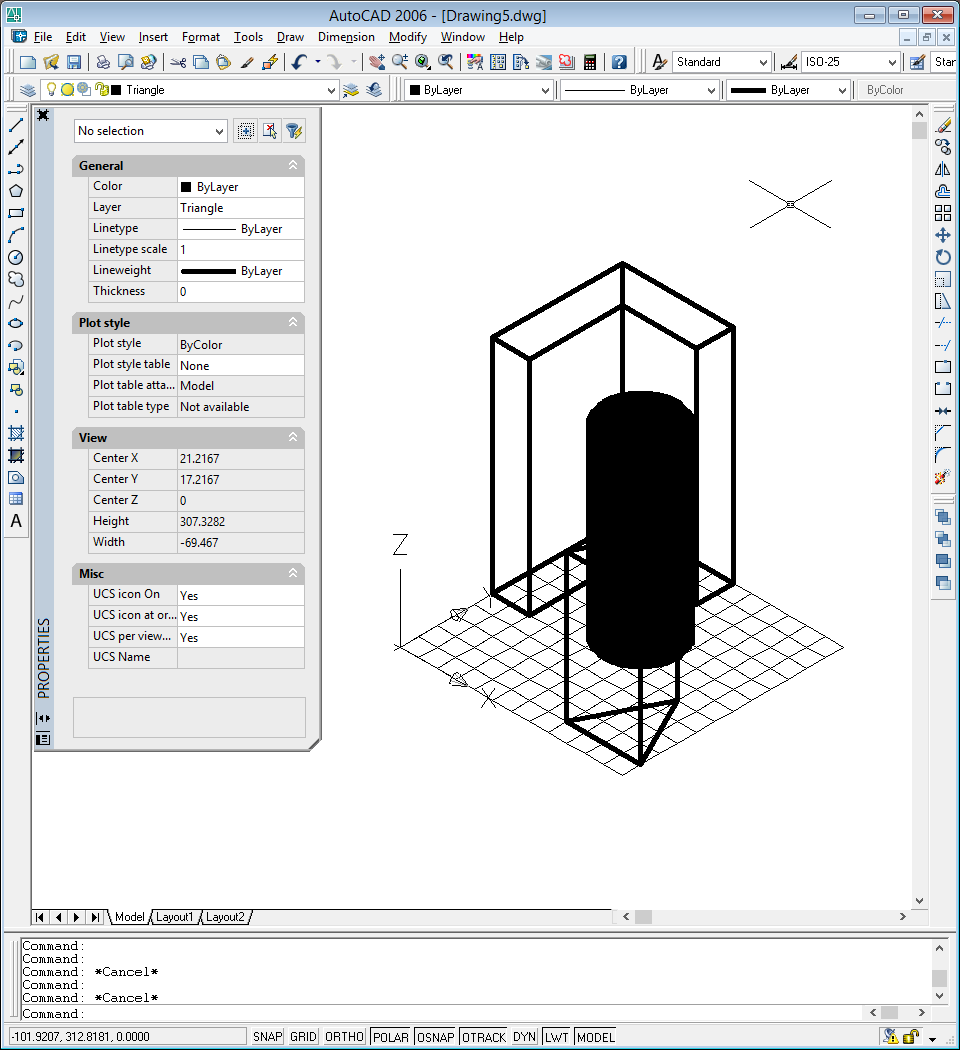
\includegraphics[width = \columnwidth]{./assets/p09.png}
					\caption{}
					\label{subfig:03-figures-3d-tall-all}
				\end{subfigure}%
				\hspace{2 \gridunitwidth}%
				\begin{subfigure}[b]{4 \gridunitwidth}
					\centering
					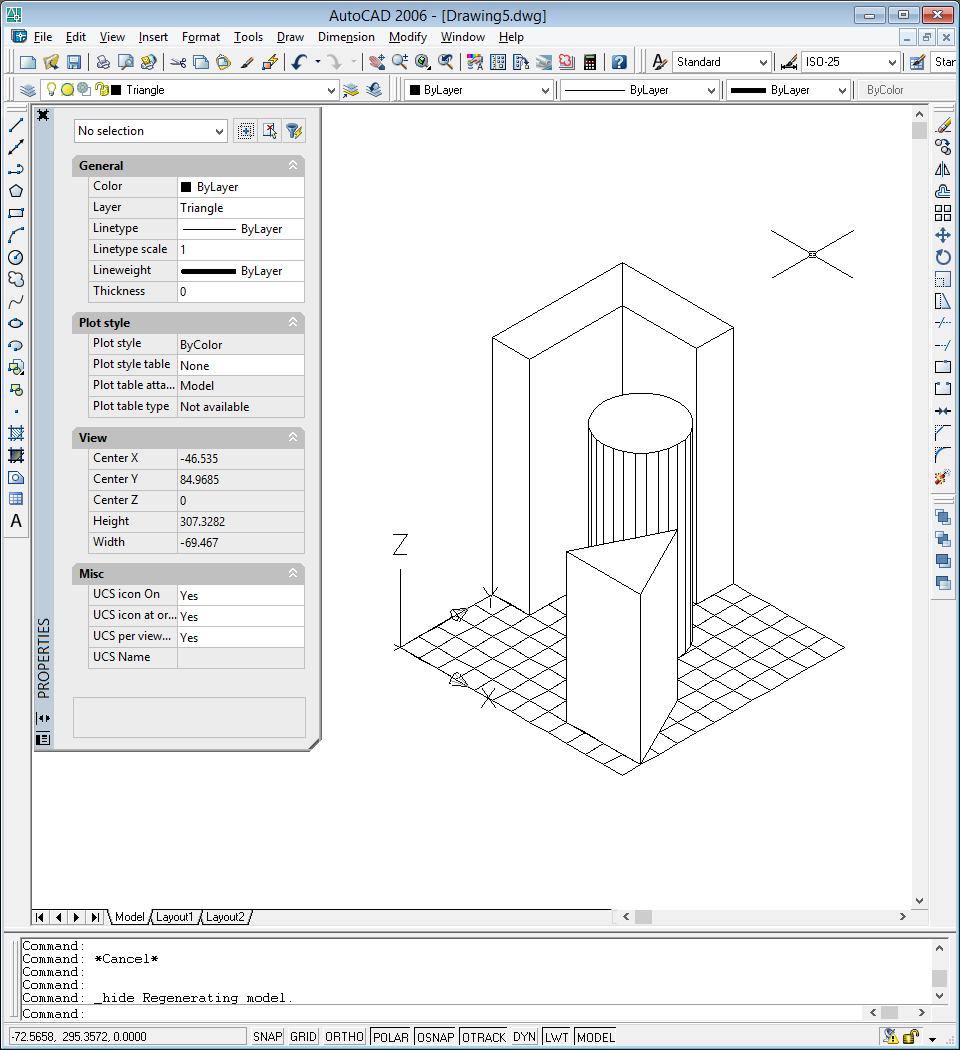
\includegraphics[width = \columnwidth]{./assets/p10.png}
					\caption{}
					\label{subfig:03-figures-3d-hidden}
				\end{subfigure}
				\caption{Побудова тривимірних зображень фігур}
				\label{fig:03-figures-3d}
			\end{figure}

			В результаті виконання вправи ми переключили режим зображення фігур на більш зручний для тривимірного моделювання, а також перетворили двовимірні фігури на тривимірні за допомогою параметра~\textenglish{Thickness}.

		\subsection{Вигляди і виглядові екрани}
			Щоб увімкнути виглядовий екран, зручний для тривимірного моделювання, оберемо пункт меню~\menu{\textenglish{View} > \textenglish{Viewports} > \textenglish {New Viewports...}} в результаті відкриється менеджер виглядових екранів~(рис.~\ref{subfig:04-viewports-01}). Оберемо у ньому зручний виглядовий екран та збережемо його під зручним ім'ям. Натискаємо кнопку~«ОК» і бачимо, що був встановлений зручний видовий екран~(рис.~\ref{subfig:04-viewports-02}).

			\begin{figure}[!htbp]
				\begin{subfigure}[t]{4 \gridunitwidth}
					% \centering
					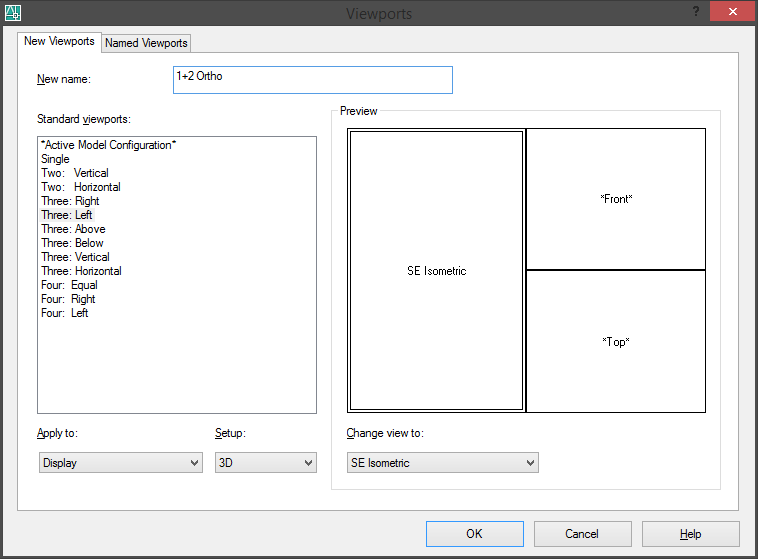
\includegraphics[width = \columnwidth]{./assets/p11.png}
					\caption{}
					\label{subfig:04-viewports-01}
				\end{subfigure}%
				\hspace{2 \gridunitwidth}%
				\begin{subfigure}[t]{4 \gridunitwidth}
					\centering
					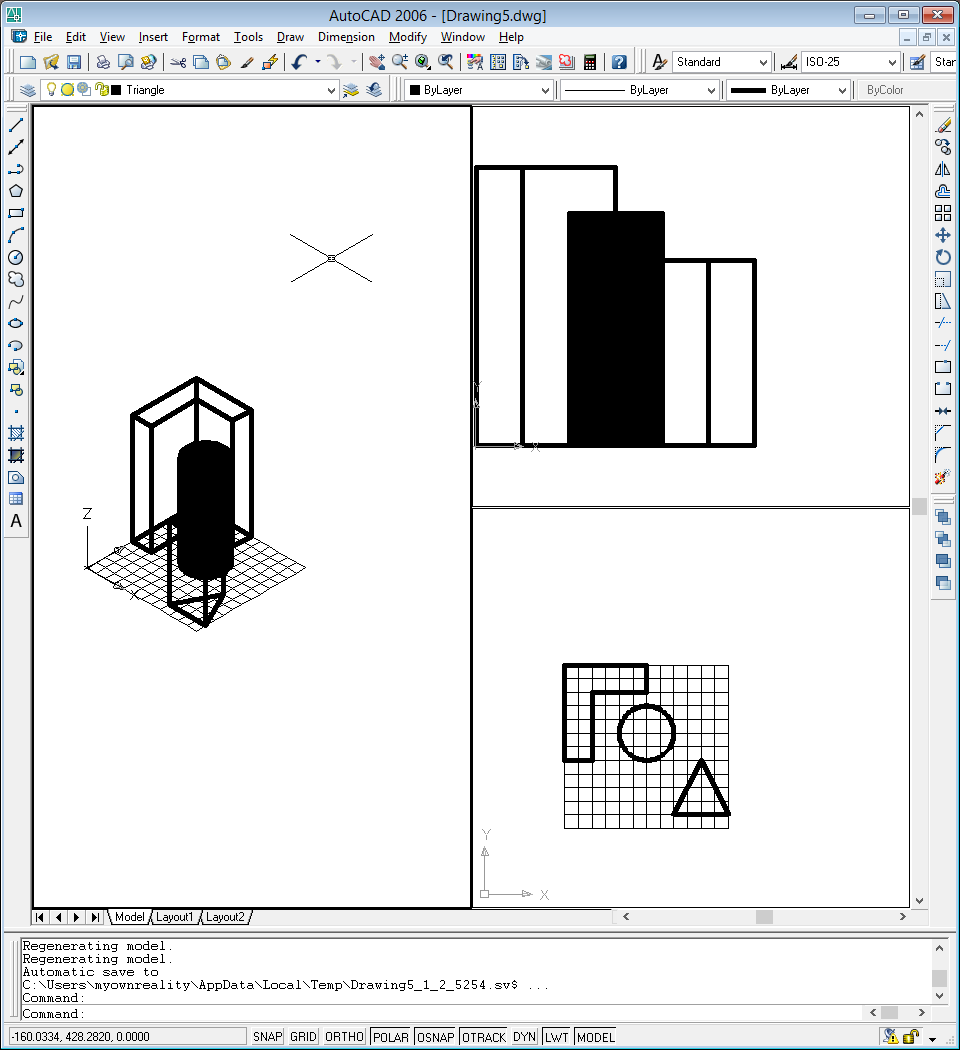
\includegraphics[width = \columnwidth]{./assets/p12.png}
					\caption{}
					\label{subfig:04-viewports-02}
				\end{subfigure}
				\caption{Встановлення видового екрану}
				\label{fig:04-viewports}
			\end{figure}

			Тепер встановимо один вигляд: виберемо пункт меню~\menu{\textenglish{View} > \textenglish{Viewports} > \textenglish{1 Viewport}}. Після цього буде показаний одновиглядовий екран~(рис.~\ref{subfig:05-viewport-single-01}). Його ракурс можна змінити у меню~\menu{\textenglish{View} > \textenglish{3D Views}} обрати найбільш зручний~(рис.~\ref{subfig:05-viewport-single-02}).

			\begin{figure}[!htbp]
				\begin{subfigure}[b]{4 \gridunitwidth}
					% \centering
					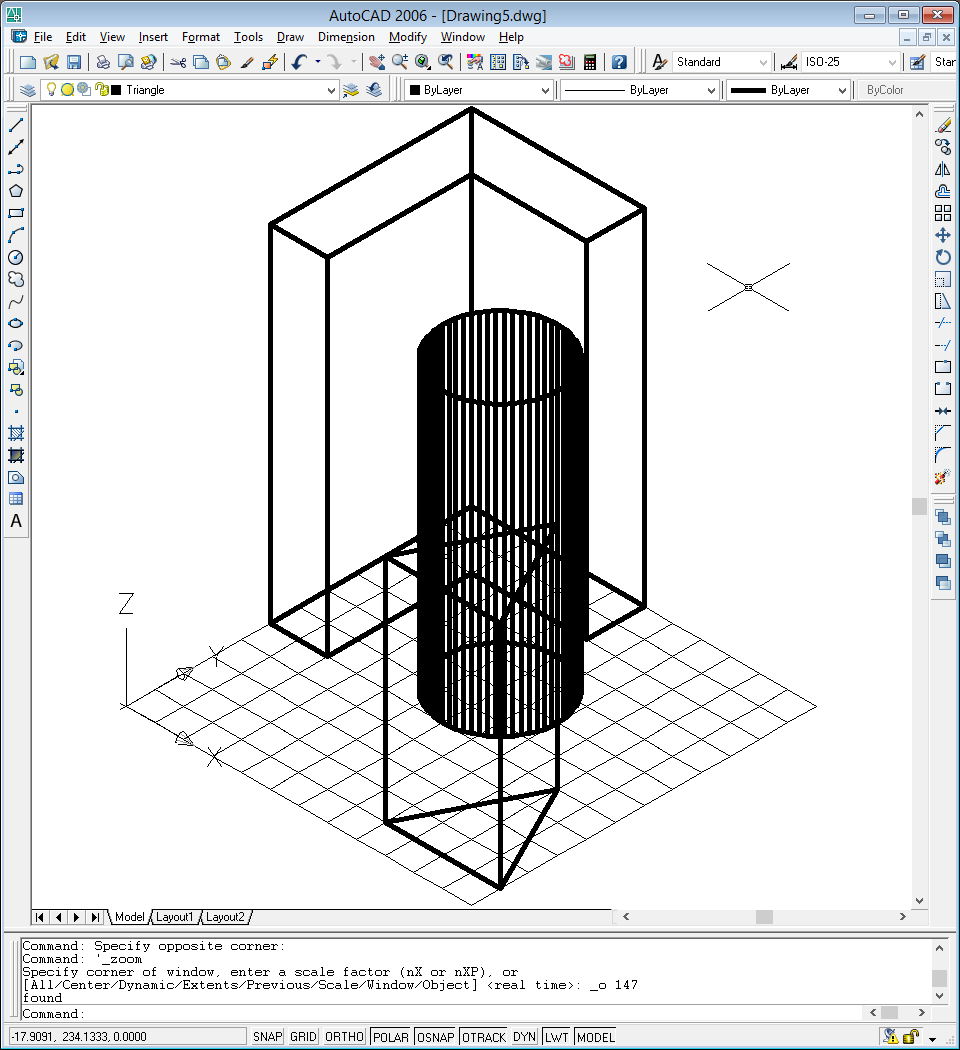
\includegraphics[width = \columnwidth]{./assets/p13.png}
					\caption{}
					\label{subfig:05-viewport-single-01}
				\end{subfigure}%
				\hspace{2 \gridunitwidth}%
				\begin{subfigure}[b]{4 \gridunitwidth}
					\centering
					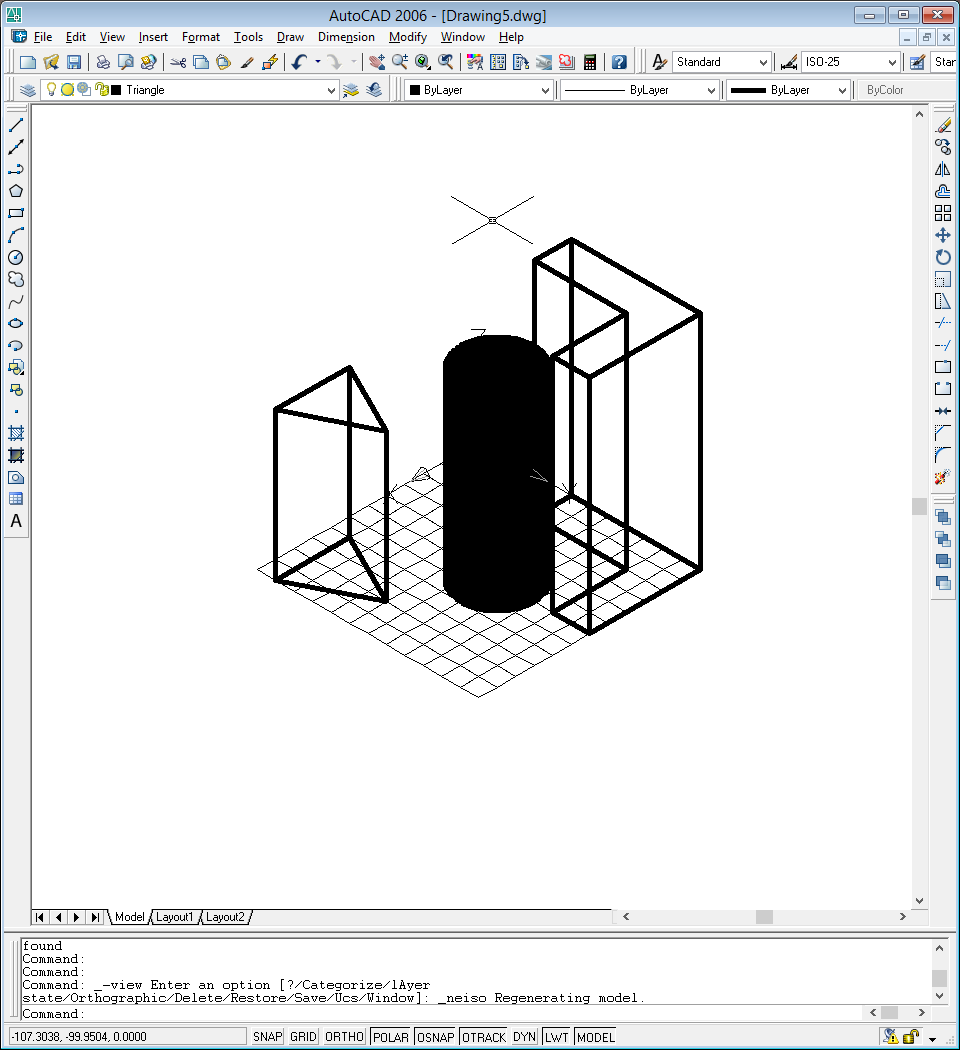
\includegraphics[width = \columnwidth]{./assets/p14.png}
					\caption{}
					\label{subfig:05-viewport-single-02}
				\end{subfigure}
				\caption{Установка єдиного виглядового екрану}
				\label{fig:05-viewport-single}
			\end{figure}

			Виконуючи вправу, ми встановили виглядові екрани і обрали їх ракурси.

		\subsection{Динамічна зміна вигляду та розфарбовування об'єктів}
			Щоб динамічно змінювати ракурс огляду тривимірних фігур, викликають команду~\acad{3dorbit}. Вона дозволяє довільно обертати фігуру у тривимірному просторі за допомогою інтерфейсу орбітального кільця~(рис.~\ref{subfig:06-dynamic-rotation-01}). Під час обертання моделі інструментом~\acad{3dorbit}, можна зафарбувати побудовані фігури, щоб вони відбивали світло. Для цього натискають праву клавішу миші і обирають пункт~\menu{\textenglish{Shading Modes} > \textenglish{Gouraud Shaded}}. Цей режим найбільш наочно відрізняє фігури, якщо кожна фігура пофарбована у різний колір~(рис.~\ref{subfig:06-dynamic-rotation-02}).

			\begin{figure}[!htbp]
				\begin{subfigure}[b]{6 \gridunitwidth - (1em / 2)}
					% \centering
					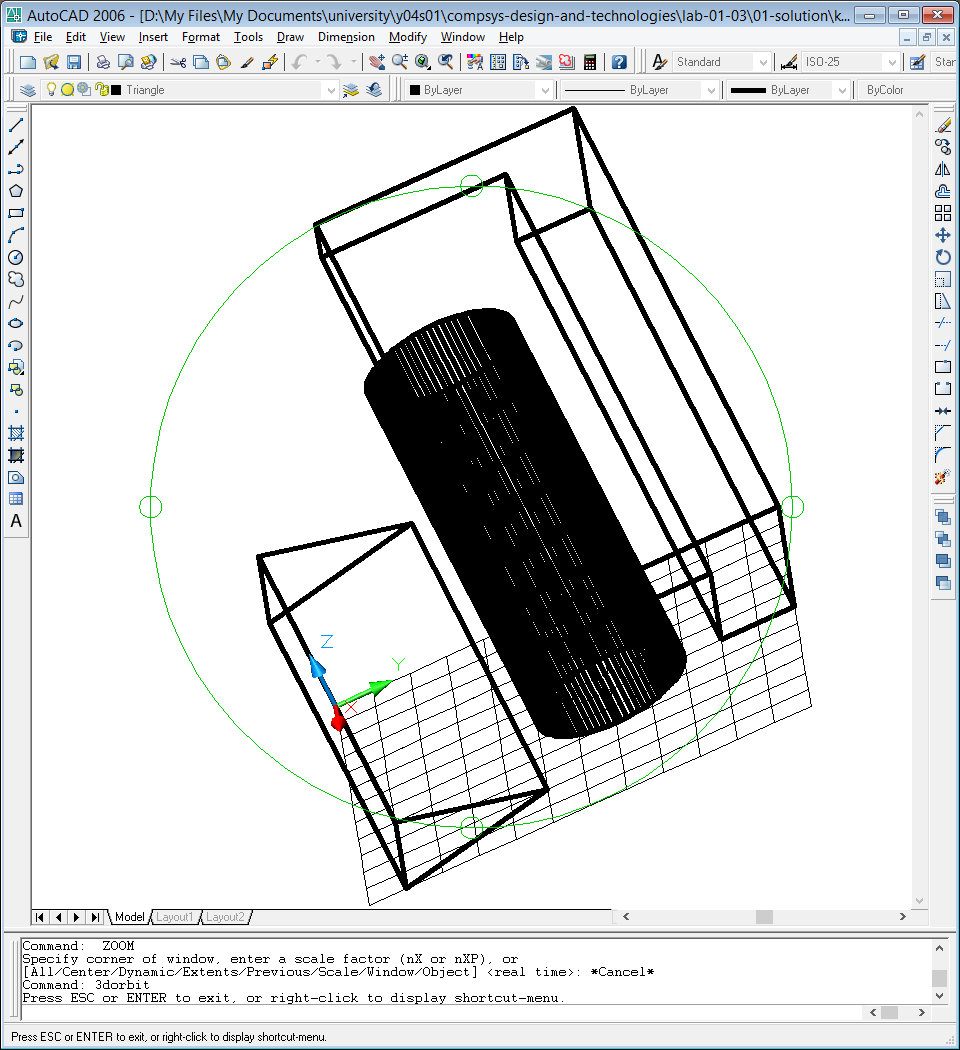
\includegraphics[width = \columnwidth]{./assets/p15.png}
					\caption{}
					\label{subfig:06-dynamic-rotation-01}
				\end{subfigure}%
				\hspace{1em}%
				\begin{subfigure}[b]{6 \gridunitwidth - (1em / 2)}
					\centering
					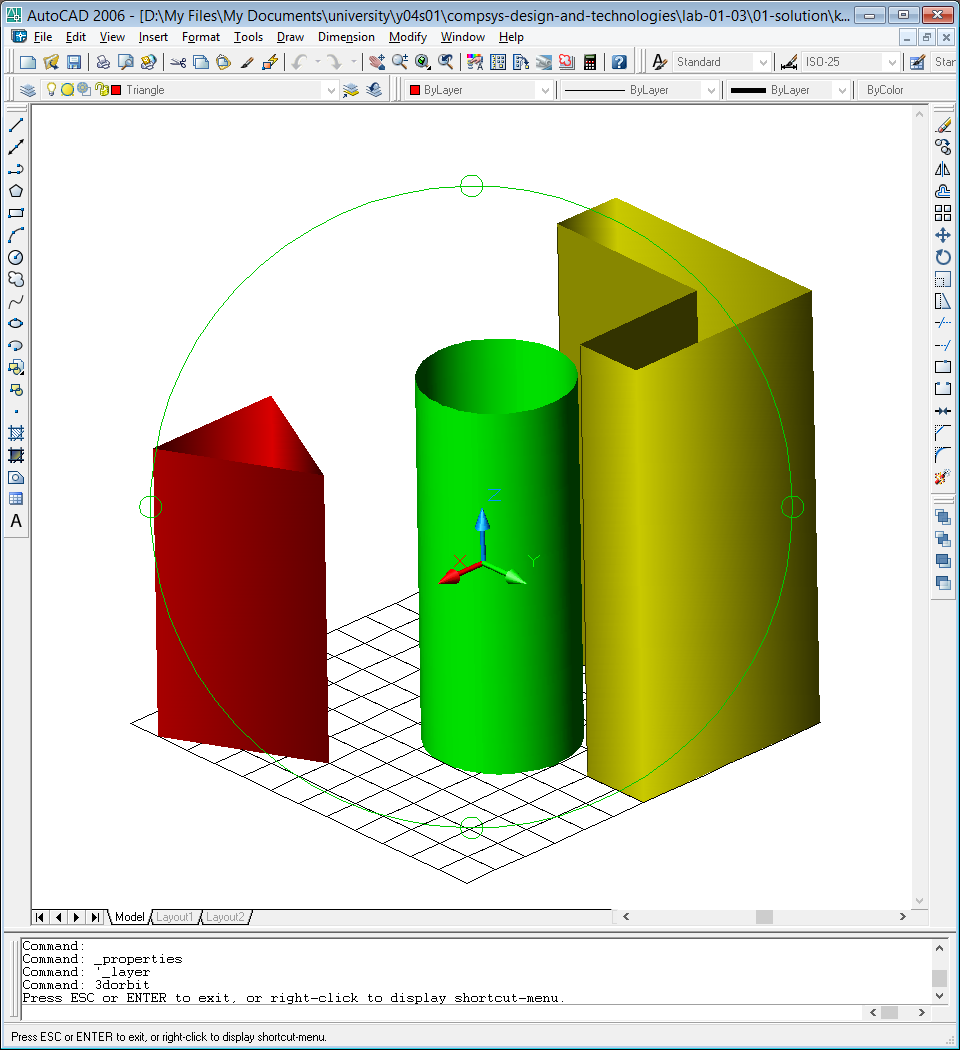
\includegraphics[width = \columnwidth]{./assets/p16.png}
					\caption{}
					\label{subfig:06-dynamic-rotation-02}
				\end{subfigure}
				\caption{Динамічна зміна вигляду і розфарбування об'єктів}
				\label{fig:06-dynamic-rotation}
			\end{figure}

		Отже, виконуючи дану вправу ми навчились змінювати вигляд тривимірних фігур, а також розфарбовувати їх, щоб більш наочно їх представляти.

	\section{Висновок}
		Виконуючи дану лабораторну роботу, ми~оволоділи технологіями відображення графічних об'єктів у тривимірному вигляді.

\end{document}
